\documentclass{article}
\usepackage[utf8]{inputenc}
\usepackage{lmodern}
\usepackage{amsmath}
\usepackage{parskip}
\usepackage{graphicx}
\graphicspath{ {./} }
\title{Hal\_3900 Proposal}
\begin{document}
\begin{LARGE}
\begin{center}
\vspace*{15mm}

COMP3900

Hal\_3900 Proposal

\rule[4.5pt]{0.61\textwidth}{0.3pt}

% also need to include email and scrum role
\begin{align*}
  \text{Ellen Oates}    \quad   &\text{z5098896} \\
  \text{Hayden Le}      \quad   &\text{z5098972} \\
  \text{Yi Wang}        \quad   &\text{z5124282} \\
  \text{Zain Afzal}     \quad   &\text{z5059449} \\
\end{align*}

\rule[4.5pt]{0.61\textwidth}{0.3pt}

x/03/2019

\end{center}
\end{LARGE}
\newpage

%-------------------------------------------------------------------------------------------------%

\section{Background}

\subsection{The Problem}
* could we survey lecturers and tutors to get an idea of the quantity of emails they get / how long they spend answering administrative questions per week? would this help our proposal?

Online learning is changing the way students access and engage with higher education. Courses with online delivery increase the flexibility and accessibility of courses by providing students with a platform to learn course content in their own time, at their own pace. Increasingly courses which are taught face to face include some online content delivery, including course materials, quizzes, online lecture recordings, and forums to ask questions and discuss the course content outside of class.   

There is a delay between when students ask a question and when they get a response, and this can vary from hours to days. Answering individual student questions via email or on the forums requires a significant amount of time for tutors, course administrators and lecturers. Often the same questions will be asked many times by different students, making it inefficient to have course staff respond to each one individually.

........ 

Some students need more learning support for course content (and don't always use the help sessions/tutorials effectively for this)
Some students need more support with lab work and assignment organisation to keep on top of due dates etc. 

* cite research about online learning from educator perspective
Lecturers and tutors want to know what their students need the most help with, to target their teaching better. Students are in different 
places with their learning and often need more individualised support to learn either the basic content, or suggestions of more advanced 
material to extend themselves. This is difficult to provide in a large class properly.


\subsection{The Existing Solution}

Currently at UNSW, learning support is provided to students through email, forums and help sessions. This is very man hour heavy, requiring countless tutors to be on hand to answer questions which of themselves are quite repetitive. In addition as these courses become larger with increasing enrollment sizes it becomes more difficult to be able to give students individual attention and personalised education. 

Another side effect of growing cohort sizes is the fact that many tutors and lecturers are forced to spend most of their time answering admin related questions and helping students to clarify their understanding, time that could be spent bettering the course and writing course material. Hiring more staff and offloading many questions to forums has been the current approach used by courses to handle this increasing load but forums are full of repeat questions and require many tutors to man them. 

This growth is becoming unsustainable and with the rise of online education platforms many students are eager to interact with course material in a more interactive meaningful way which works with their scedule. Waiting for a tutor to respond to them often creates a distance between the inital question and the answer which limits the effectivenes of a response. That is if the tutor finds time to respond at all. 

In some areas of education chat bots have been deployed which interact with students in meaningful ways out of class hours (create a reference to https://botsify.com/education-chatbot) and some have even been created to answer higher education questions (reference https://www.canberra.edu.au/about-uc/media/newsroom/2018/february/students-make-new-friend-in-lucy-the-chatbot). However these tools are not able to me easily mapped to a unsw university course, it's administration, assessments and can not utilise archives of previous iterations of the course to learn common questions and issues.


\subsection{Our Solution}

The goal is to create a chat bot companion for students to enhance their learning experience. The chat bot will provide students with learning support by responding to their questions about course administration and the content they are learning, in real time, and monitoring their understanding of the course content with follow up questions.

The chat bot will assist students with revision, and will provide organizational support by keeping students informed of their grades and upcoming due dates.

The chat bot will enhance course delivery by keeping staff informed of their students' learning needs and frequently asked questions. It will reduce the load on lecturers, tutors and course administration staff by answering many of the questions that students have, allowing them to focus on the overall delivery of the course. 


\subsection{Technical Details}

For this bot we will be building servals layers to form our technical stack.

\begin{itemize}
  \item A frontend will be build in Vue.js interaction with a Node.js backend via Websockets to provide a frontend to interact with the chatbot
  \item Dialogflow will be used to parse user input and provide the natural language processing aspect of this project
  \item Actions will be passed to the knowledge base of the bot, which built ontop of tensor flow which will utilise machine learning to classify data and form connections between a input query and the relevant data points.
  \item Data will be stored in s3 buckets
  \item Docker will be utilised to unify the several layers of this application into a holistic program. 
\end{itemize}

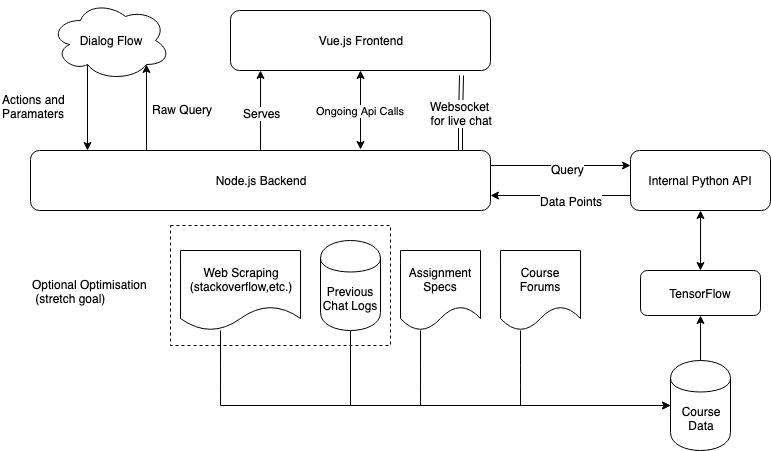
\includegraphics[width=\textwidth]{architecture_diagram.png}

The scope of this program is to have a bot which can answer most basic administration questions such as when assignments are due and has at least a 50\% success rate with responding to direct questions with a simple data point response i.e "how do you print with no new line in python" should respond with "you can use sys.stdout.write". In addition the bot should have the ability to quiz students from a lecturer defined set of questions, a stretch goal would be for the bot to autogenerate these.


\section{Epics}

\subsection{Answers administrative questions about course}

The chatbot will play the role of “Course administrator” and help students to efficiently manage their course. It will answer questions about the following information:
\begin{itemize}
  \item Assignments management: includes the requirements of assignments, relevant dates (release date, deadlines), weighting, and materials provided by the lecturer.
  \item General information: includes locations of the lectures, timetables, information of lecturers (e-mails, details etc.), notices, course schedule, teaching strategies, assumed knowledge, student learning outcomes and homepage address.
  \item Assessment details: includes items with their weightings, due dates, and calculation method of the final score.
  \item Textbooks: includes the list of textbooks as well as pages addresses of them if it is.
\end{itemize}

This epic aims to help students to access the course administrative information, which is mostly gained from the course outline. It will be limited to answer questions about existing information which is already provided by the course homepage. Questions about further information such as detailed course context will not be included in this epic.

This epic has an estimated difficulty score of 4/10, due to the workload is not large, and a time estimate of 5 units.


\subsection{Answers questions about course content}
This is the next major category that student questions will fall into. Although questions in this category may be less common for course administrators compared to queries such as "when is assignment 2 due?", they make up a significant proportion of questions directed to tutors. Implementing this feature in this chat bot will remedy a number of problems that this poses.

\begin{itemize}
  \item Gives immediate answers to students, eliminating the need to wait for tutors' responses.
  \item Reduces workload of tutors, who are typically only paid for one hour of associated work.
  \item Can answer questions beyond the scope of tutors' knowledge.
  \item Discourages plagiarism by providing an officially endorsed information bank.
  \item Offers an outlet for shy students to ask individual questions.
\end{itemize}

The bot's knowledge base can be built from a number of sources. Apart from manual input, this can also include information scraped from appropriate sources such as course syllabus, lecture slides and past assignment submissions.

Information not directly related to the course content should be considered out of scope. However as there is no clear divide between what constitutes course content and what doesn't, there will be some degree of leniency as to what is included.

As one of the primary features, it has an estimated difficulty score of 8/10 with a time estimate of 5 time units. That said, the actual implimentation is not unlike that of epic 1, so there is potential for this epic to be developed alongside epic 1 as the functionality may be shared.


\subsection{Meaningfully quizzes and interacts with students}
The chatbot will be continuous trained and personalized to fit student’s needs, as well as provide meaningful quizzes to students. Therefore, the chatbot will provide answers with increasing accuracy, meanwhile, students can conveniently examine their selves, and compensate their weakness

The epic includes 2 important fields:
\begin{itemize}
  \item Statistics: the chatbot will gather questions which the student has asked, to analyze the learning status of the student in fields included by the course. According to the analysis, the weakness of the student will be figured out to help formed quizzes content. Those quizzes will be provided when they were asked. On the other hand, a statistics conclusion will also be provided to students, which will be helpful for their final review.
  \item Personalization: the chatbot will interact with the student and trained itself according to the feedback. This process will help students to personalize their chatbots, to make the chatbots be more familiar with the users’ language habits. Therefore, chatbots can provide progressively more accurate answers. 
\end{itemize}

The scope of the epic is limited to face to only one student, and all happened conversations will be treated as information from one person. Moreover, the quizzes questions will from a preset database, further questions will not be included.

This epic has an estimated difficulty score of 7/10, and a time estimate of 8 units.


\subsection{Informs course admin/staff about cohort}

This feature will allow the chat bot to maintain information about the questions users are asking and the performance of users in the excersizes the bot sets forward. This will be accessable from the admin web interface available to course staff.

The main metrics that should be captured for a requested time frame are
\begin{itemize}
  \item A list of the most common questions asked and their relative frequency
  \item A list of missed questions
  \item A list of the questions or triggers which the bot had a low satisifaction rate for
  \item A breakdown of every topic covered and it's retention rate amongst users (derived from interactive quizzing)
  \item General statistics on the bot's usage rate, uptime and the average computation time taken for a response
\end{itemize}

The web interface will provide the ability to 
\begin{itemize}
  \item View interactive sortable tablular data for the followed metrics
  \item View certain data such as usage rate and computation time as a graph against time
  \item Export the metrics as csv or json
  \item Register admin staff to be notified by email when certain conditions are met, i.e missed question rate rises past 50%
\end{itemize}

Out of scope will be any more advanced interaction with the data other then simple tabulation and graphing against time. More forms of data visualisation should be derferred to specialist tools. 

In addition this is simply to inform users of the bots performance and will not provide features to adjust the paramaters of the bot, this will be defered to the second epic involving the bot's interaction with course content. 

This will be a somewhat difficult set of features to implement, it's estimated difficulty score is 7/10 with a time estimate of 5 time units.


\subsection{Learns for more then one course without needing massive config} % this title needs work tbh

The chat bot is able to adapt to other courses provided at UNSW and start providing student support quickly 
Course admin gets a really easy setup wizard?? think about.... 
(make it plug and play basically)   will improve the wording on this


\section{Epic Selection}

Of the proposed epics, the following epics will be delivered in the final release:
\begin{itemize}
  \item Answers administrative questions about course
  \item Answers questions about course content
  \item Learns for more then one course without needing massive config
\end{itemize}

Considering the goals of this project, these epics clearly outline the core functionality that should be achieved to deliver a minimum viable product. The main goal is to have a chat bot that students can direct questions to, and the epics were chosen accordingly.

The first two epics that were chosen directly correlate with the intended final outcome. Although the third epic is not directly related to this cause, it is an important feature required to perform the initial configuration of the chat bot, which is required to allow it to function normally.

The remaining epics are:
\begin{itemize}
  \item Meaningfully quizzes and interacts with students
  \item Informs course admin/staff about cohort
\end{itemize}

These epics go hand in hand to an extent, and while the features they provide are definitely useful, they are not essential to the basic functionality and upkeep of the chat bot. As such, they will be considered stretch goals which will be implemented if the scope of the project allows.


\section{Summary}

This project aims to deliver a chat bot that students can use as an assistant while taking certain courses. It will be implemented as a web application to provide an easy-to-use interface and developer-friendly code base to allow for extensibility. 

\section{Glossary}

\begin{align*}
  \text{Missed Question}    \quad   &\text{A question which the chat bot was not able to answer}
\end{align*}

\end{document}
